
%%%%%%%%%%%%%%%%%%%%%%% file typeinst.tex %%%%%%%%%%%%%%%%%%%%%%%%%
%
% This is the LaTeX source for the instructions to authors using
% the LaTeX document class 'llncs.cls' for contributions to
% the Lecture Notes in Computer Sciences series.
% http://www.springer.com/lncs       Springer Heidelberg 2006/05/04
%
% It may be used as a template for your own input - copy it
% to a new file with a new name and use it as the basis
% for your article.
%
% NB: the document class 'llncs' has its own and detailed documentation, see
% ftp://ftp.springer.de/data/pubftp/pub/tex/latex/llncs/latex2e/llncsdoc.pdf
%
%%%%%%%%%%%%%%%%%%%%%%%%%%%%%%%%%%%%%%%%%%%%%%%%%%%%%%%%%%%%%%%%%%%


\documentclass[runningheads,a4paper]{llncs}

\usepackage{amssymb}
\setcounter{tocdepth}{3}
\usepackage{graphicx}
%\usepackage{comment}
\usepackage{tikz}
\usepackage{float}
\usepackage{subfig}

%\usepackage{subfloat}
\usepgflibrary{arrows}
\usetikzlibrary{arrows,decorations.pathmorphing,backgrounds,fit}
\usetikzlibrary{shapes.geometric}
\usepgflibrary{shapes.geometric}
\usetikzlibrary{shapes.symbols}
\usepgflibrary{shapes.callouts}
\usetikzlibrary{shapes.callouts}

\usetikzlibrary{through} 
%%\usetikzlibrary{arrows,bac

\usepackage{url}

\urldef{\mailsa}\path|{u.berger, p.d.james, m.roggenbach, m.seisenberger}@swansea.ac.uk|
\urldef{\mailsb}\path|ajlawrence@acm.org|
\newcommand{\keywords}[1]{\par\addvspace\baselineskip
\noindent\keywordname\enspace\ignorespaces#1}

\begin{document}
\mainmatter  % start of an individual contribution
% first the title is needed
\title{Modelling and Analysing the European Rail Traffic Management System\\in Real-Time Maude}
% a short form should be given in case it is too long for the running head
\titlerunning{Modelling and Analysing ERTMS in Real Time Maude}
% the name(s) of the author(s) follow(s) next
%
% NB: Chinese authors should write their first names(s) in front of
% their surnames. This ensures that the names appear correctly in
% the running heads and the author index.
%
\author{Andrew Lawrence\thanks{Supported by Siemens Rail Automation and EPSRC} \and Ulrich Berger \and Phillip James \and \\ Markus Roggenbach \and  Monika Seisenberger}
%
\authorrunning{Lawrence, Berger, James, Roggenbach, Seisenberger}
% (feature abused for this document to repeat the title also on left hand pages)
% the affiliations are given next; don't give your e-mail address
% unless you accept that it will be published
\institute{%%Department of Computer Science, \\ 
Swansea University, UK\\
\mailsb \\
\mailsa
}
%
% NB: a more complex sample for affiliations and the mapping to the
% corresponding authors can be found in the file "llncs.dem"
% (search for the string "\mainmatter" where a contribution starts).
% "llncs.dem" accompanies the document class "llncs.cls".
%
\toctitle{Modelling and Verifying the European Rail Traffic Management System in Real Time Maude}
\tocauthor{Authors' Instructions}

\maketitle

\begin{abstract}
We report on experimental work towards modelling the ERTMS in Real
Time Maude and performing qualitative analysis for safety and
quantitative analysis for system performance.
\end{abstract}


\section{Introduction}
The European Rail Traffic Management System (ERTMS) is a next
generation train control system, loosely specified in
\cite{SRS}. Traditionally, the railway has been constructed from
discrete entities such as signals, \emph{track circuits} for train
detection, and \emph{interlockings} that use propositional equations
to guarantee train safety. In contrast, the ERTMS deals with
continuous data that allows for a finer grain of control over
railway traffic. In ERTMS, a \emph{radio block centre} (RBC) grants each
train a block of track, called a \emph{movement authority}, in which
the train is allowed to move, see Figure \ref{fig:ertms}. ERTMS requires trains to have
on-board equipment that ensures trains to brake in time. While the
correctness of traditional interlocking systems is relatively well
understood \cite{Interlockings}, it is ongoing research to
verify ERTMS based systems for safety properties such as collision freedom due to
the involvement of continuous data. Furthermore, it is an open field of
how to substantiate the claim that the ERTMS approach offers a higher
performance of the railway compared to traditional railway control.
\begin{figure}
\centering
\includegraphics[height=5cm]{etcs}
\caption{Overview on ERTMS, level 2}
\label{fig:ertms}
\end{figure}





\section{Methodology}
We first model the ERTMS as a system of hybrid automata and establish
that these automata are non-zeno, i.e., every finite initialised
trajectory in the labelled transition system defined by the automaton
has an infinite trajectory of which it is a prefix in the set of
divergent initialized trajectories in the automaton. This property has
been manually proven in a generic way for the automaton representing a
train. For the other components, namely the interlocking and the radio
block centre, the automata are non-zeno as they do not include timing
conditions.

Real-Time Maude is an extension of Full Maude which supports the
specification to real-time and hybrid systems. Offered techniques
include simulation and time-bounded LTL model checking for
verification of timed properties. We use the Real-Time Maude system
\cite{RTMaude} for the specification of ERTMS, and the Maude linear
temporal logic (LTL) model checker \cite{LTLmodelchecker} for
verification.  In our model, speed, acceleration, braking behaviour
and track length are integral parts. This allows us to specify and
prove safety properties, such as collision freedom, over the system
and to study how the system performs over time via execution of the
specification as a simulation.

\begin{figure} [h!]\begin{center}
\subfloat[Pentagon Example]{
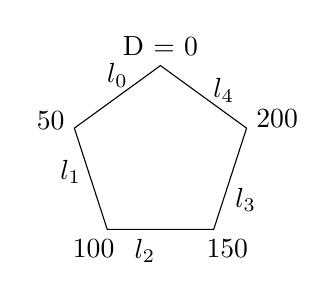
\begin{tikzpicture}[node distance = 2.3cm, scale = 0.7]
\node (A) [draw,regular polygon, regular polygon sides=5, minimum size=2.3 cm,outer sep=0pt] {};
\foreach \n in {1,...,1} {
    \pgfmathtruncatemacro{\value}{(\n - 1) * 50};
    \pgfmathtruncatemacro{\valuem}{(\n - 1)};
    \node at (A.corner \n) [anchor=360/5*(\n-1)+270] {D = \value};
    \node at (A.side \n) [anchor = 360/5 *(\n-1) +270] {$l_{\valuem}$};
}
\foreach \n in {2,...,5} {

    \pgfmathtruncatemacro{\value}{(\n - 1) * 50};
    \pgfmathtruncatemacro{\valuem}{(\n - 1)};
    \node at (A.corner \n) [anchor=360/5*(\n-1)+270] { \value};
    \node at (A.side \n) [anchor = 360/5 *(\n-1) +270] {$l_{\valuem}$};
}
%%%\node (B) [draw, rectangle, rotate = 36] at (-1.9,2.6) {Train A};
%%%\node (C) [draw, rectangle, rotate =72] at (3,-1) {Train B};
\end{tikzpicture} 
}\hspace{10pt} \label{fig:pentagon}
\subfloat[Junction Example]{
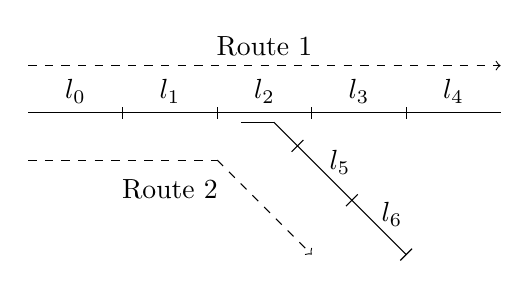
\begin{tikzpicture}[node distance = 3cm, scale = 0.6]
\draw (0,0) -- (10,0);
\foreach \n in {1,...,5} {
  \pgfmathtruncatemacro{\valuem}{(\n - 1)};
    \node () [above] at (\n *2 -1,0) {$l_{\valuem}$};
}
\foreach \n in {2,...,5} {
  \pgfmathtruncatemacro{\valuem}{(\n - 1)};
    \draw (\valuem *2, -0.125) -- (\valuem *2, 0.125) ;
}
\draw (4.5,-0.2) -- (5.2, -0.2);
\draw (5.2,-0.2) -- (8,-3);
\draw (5.575,-0.825) -- (5.825,-0.575);
\draw (6.725,-1.975) -- (6.975,-1.725);
\draw (8.125,-2.875) -- (7.875, -3.125);
\node () [] at (6.6,-1.05) {$l_5$};
\node () [] at (7.7,-2.15) {$l_6$};
\draw [->,dashed] (0,1) -- (10,1);
\node () [above] at (5,1) {Route 1};
\draw[dashed] (0,-1) -- (4,-1);
\draw[->,dashed] (4,-1) -- (6,-3);
\node() [below] at (3,-1.2) {Route 2};
\end{tikzpicture} 
}\label{fig:junction}
\caption{Case Studies}
\end{center}
\end{figure}


\section{Case Studies} 
We first formalise a simple example railway in
the shape of a pentagon (see Fig.~2~(a)) with two trains, one slower
than the other, an interlocking, an RBC and five track segments
$\{l_0, \ldots, l_4 \}$ as four hybrid automata to capture the
behaviour of the system. This example demonstrates how the ERTMS
system deals with a length of track containing multiple trains that
are controlled by an RBC and interlocking. We proceed to model
this example in the Real Time Maude system as an object
orientated specification capturing the message passing and
communications between the different components of the system. This
specification is executed to simulate the behaviour of the modelled
railway. The faster train can be observed catching up with the slow train
and then braking and waiting for authorisation before moving off
again. We verify that the movement authorities of the two trains do
not overlap, expressed by safety properties of the form ``it
is globally true that if both trains are behind their movement
authorities then either train1's movement authority is behind train2's 
or vice versa".

As a second case study we model an open system, a simple junction (see
Fig.~2~(b)) which contains a single point and two routes each
consisting of five track segments. Trains are inserted onto the
railway line according to a schedule by a controller object. Each train is also assigned a
given route which they must follow. This example demonstrates the
behaviour of ERTMS with respect to two further important constructs in
the railway domain namely routes and points. It enables us to analyse
the throughput of the ERTMS over a junction where one train
must wait for the point to become available. The Maude LTL model
checker is then applied to verify that a point does not move in a
given movement authority, a safety property that is essential for the
prevention of derailment. 

\section{Formalisation} In the following we show some aspects
of our formalisation to give a hint on how we modelled in Maude the
interplay between trains, the interlocking and the radio block
centre. Here, we presume some familiarity with Maude as an introduction
to its language constructs is beyond the scope of this paper.


In particular, we show the structure of the train class, and formulate
a simple safety condition to be model checked.  Classes for the radio
block processor and the interlocking are defined similarly.

Real time Maude allows us to compose objects and messages 
together to form a subsort of \texttt{System} called a \texttt{Configuration}.

\begin{verbatim}
mod CONFIGURATION is  
    *** basic object system sorts  
    sorts Object Msg Configuration .  
 
    *** construction of configurations  
    subsort Object Msg < Configuration .  
    op none : -> Configuration [ctor] .  
    op __ : Configuration Configuration -> Configuration  
         [ctor config assoc comm id: none] .
\end{verbatim}

Here, the composition operation for configurations is commutative, and
the order of objects and messages in a configuration does not
matter. Inspired by \cite{delta} we use an operator $\delta$ which describes
how a distributed system evolves over time. In particular, it ensures
that messages (which cannot be part of an object configuration)
between the various components are read. 

\begin{verbatim}
op delta : Configuration -> Configuration [frozen] . 
var OCREST : ObjectConfiguration .
vars CON1 CON2 : NEConfiguration .
rl [timetrans] : {OCREST} => {delta(OCREST)} in time 1 .
rl [delta1] : delta(CON1 CON2) => delta(CON1) delta(CON2) .
\end{verbatim}

We model the train class to have a state that can range over one of four
possibilities: constant speed, accelerating, braking, and
stopped. We further include current position,
speed, acceleration, movement authority, current track segment, and
maximal speed, and specify its behaviour with appropriate rules
(omitted).

\begin{verbatim}
sort TrainState .
ops  cons acc stop brake :  -> TrainState [ctor] .
\end{verbatim}

\begin{verbatim}
class Train | state : TrainState, dist : Nat, speed : Nat, 
              ac : Nat,  ma : Nat, tseg : Nat , maxspeed : Nat .}
\end{verbatim}

To simulate a run of \texttt{train1} we specify:

\begin{verbatim}
(trew {< train1 : Train | state : acc, dist : 0, speed : 0, 
   ac : 1, ma : 100, tseg : 0 , maxspeed : 5 >} in time <= 30 .)
\end{verbatim}

To prove safety, we apply the Maude LTL Model checker, which does so-called 
on-the-fly model checking where we need to define an appropriate 
satisfaction relation. The safety properties we have checked are typically of the 
form: if train1 is behind its movement authority and train2
is behind its movement authority, then there is no overlap of 
movement authorities. 

%Finally, we define a property \texttt{nomaoverlap1(O1,O2)} as follows: 

\begin{verbatim}
     eq {REST < O1 : Train |  dist : D1 , ma : M1 > 
              < O2 : Train |  dist : D2 , ma : M2 >} 
     |= nomaoverlap1(O1',O2') = (O1 == O1') and (O2 == O2') 
                                and noolap1(D1,M1,D2,M2) .} 
\end{verbatim}

where 

\begin{verbatim}
      eq noolap1(D1,M1,D2,M2) =  
         (D1 <= M1 and D2 <= M2) implies (M1 <  D2 or M2 < D1) .  
\end{verbatim}

\begin{verbatim}
(mc initstate |=t [] nomaoverlap(train1,train2) in time <= 30 .) 
\end{verbatim}

\section{Results \& Future Work.} Though the presented case studies are
of a simple nature, they demonstrate that our modelling approach works:
safety properties can be formulated and verified in reasonable time
via model-checking, performance can be studied via simulation. 

\bigskip

\begin{figure}[H]
\begin{center}
\includegraphics[scale=0.34]{t1graph} 
\includegraphics[scale=0.34]{t2graph} 
\end{center}
\caption{Train speed / distance over time -- Pentagon example}
\end{figure}

Fig.~3 shows such a simulation for the case of the Pentagon example
with two trains, where a slow train (train 1) is followed by a fast
train (train 2). As one can see on the dashed curves, the slow train
forces the fast train to make regular speed adaptions, and in this
sense dominates the system. At the end of each track, the slow train
requests a new movement authority, until this is granted the train has
to slow down. The fast train however, has to slow down more often as
it is hindered in its progress by the slow train ahead. The ERTMS was
introduced to improve exactly this kind of behaviour by opening up the
possibility to add a management layer that provides a strategy over what
kind of movement authority shall be provided to a train. In our
example, for instance the speed profile for the fast train could
always be limited to a speed of 4.

It is future work to study larger, realistic examples in order to see
if the approach scales. This might involve the development of
abstractions, and extensions of our modelling to allow us to to
establish performance properties as theorems.

Part of this work has been presented in a talk at WADT 2014
(\url{http://wadt2014.cs.ovgu.de} and appeared (as an abstract) in the
electronic pre-proceedings of this workshop (available on the WADT
webpage).

\medskip

\noindent \textbf{Acknowledgement.} 
The authors would like to thank S. Chadwick from Siemens Rail Automation for his support and encouraging feedback.

%

\begin{thebibliography}{}

\bibitem{Interlockings} Chadwick, S. , James, P. Kanso, K., Lawrence,
  A. Moller, F., Roggenbach, M., Seisenberger, M. and Setzer, A.:
  Verification of solid state interlocking programs. In SEFM'13, LNCS 8368, Springer 2014.

\bibitem{LTLmodelchecker} Eker, S., Meseguer, J., and
  Sridharanarayanan A.: The Maude LTL Model Checker and Its
  Implementation. In SPIN'03, LNCS 2648, Springer 2003.

\bibitem{delta} {\"O}lveczky, P. C., Thorvaldsen. Formal {M}odelling and {A}nalysis of the {OGDC} {W}ireless {S}ensor {N}etwork {A}lgorithm in {R}eal-{T}ime {M}aude.
In FMOODS'07, LNCS 4468, pages 122-140. Springer 2007.

\bibitem{RTMaude} {\"O}lveczky, P. C. and Meseguer, J.: Specification
  and Analysis of Real-Time Systems Using {R}eal-{T}ime {M}aude. In
  FASE'04. LNCS 2984, Springer 2004.

\bibitem{SRS} {International Union of Railways}: {ETCS} System Requirements Specification (SRS) ver. 2.3.0, 2006.




\end{thebibliography}
\end{document}
\begin{comment}

\textbf{ERTMS. }The ERTMS system consists of 3 main components; the radio block centre, the interlocking and the train.  \\
\textbf{Formalisation as Hybrid Automata: }\\
\textbf{Modelling and Verification in Real Time Maude: } 
If the sections of track in which the trains are allowed to move do not intersect then the ERTMS system is safe in this particular instance.
$\mathbf{G}(\mathit{D}_1 \leq \mathit{MA}_1 \wedge \mathit{D}_2 \leq \mathit{MA}_2) \to \mathit{MA}_1 <  \mathit{D}_2 \vee \mathit{MA}_2 < \mathit{D}_1$.
\end{comment}
%
